\documentclass{article}
\usepackage{amsmath}
\usepackage{amssymb}
\usepackage[pdftex]{graphicx}
\usepackage[framed,numbered,autolinebreaks,useliterate]{mcode}
\lstset{breakatwhitespace=false}
\usepackage{pgfplots}

\pdfpagewidth 8.5in
\pdfpageheight 11in
\topmargin -1in
\headheight 0in
\headsep 0in
\textheight 8.5in
\textwidth 6.5in
\oddsidemargin 0in
\evensidemargin 0in 
\headheight 50pt
\headsep 0in
\footskip .75in

\title{STA 601 - Lab 4}
\author{Kedar Prabhudesai}
\date{September 27, 2013}

\begin{document}
\maketitle

\begin{enumerate}
\item I implemented the Rejection Sampling algorithm in MATLAB (code attached below). However, I used a slightly different approach. Here are the steps:
\begin{itemize}
\item Draw a Sample $X$ from the Envelope Distribution
\item Now, draw a sample $Y \sim U[0,f(X)]$, where $f(.)$ is the pdf of Envelope Density.
\item Check if $Y \leq g(X)$, where $g(.)$ is the target density from which we desire to sample. 
\item If the above condition is satisfied, accept $X$, otherwise reject $X.$
\end{itemize}

Here are results using a $Uniform[0,1]$ envelope density. Histogram of 10000 samples.\\

\begin{left}
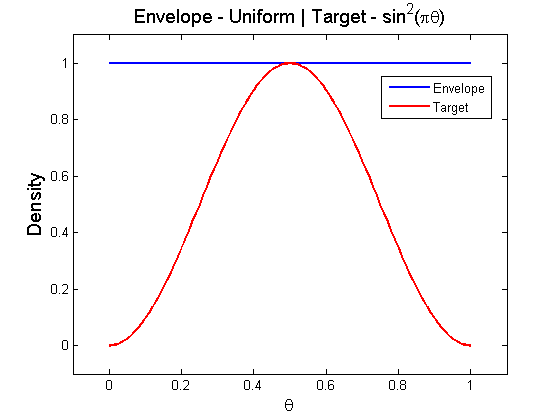
\includegraphics[scale=0.5]{Uniform.png}
\end{left}
\begin{right}
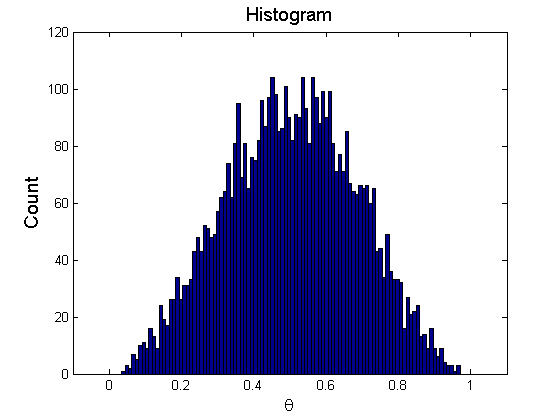
\includegraphics[scale=0.5]{UniformHist.png}\\
\end{right}

\pagebreak

\item The envelope density should be greater than or equal to the target density over the support. I chose Normal density, $\mathcal{N}(\mu,\sigma^2),$ $\mu=0.5$; $\sigma^2=0.04.$ Then I truncated the density between $(0,1).$ I get the following results:\\

\begin{left}
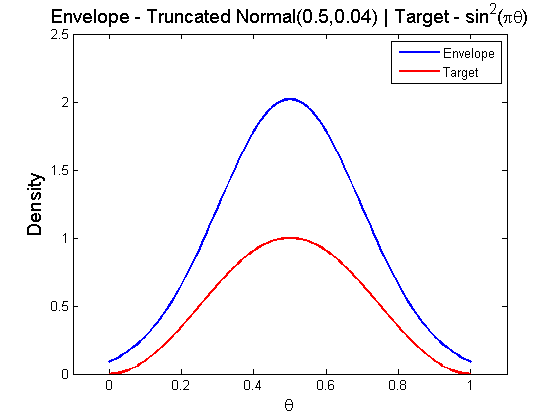
\includegraphics[scale=0.5]{Gaussian.png}
\end{left}
\begin{right}
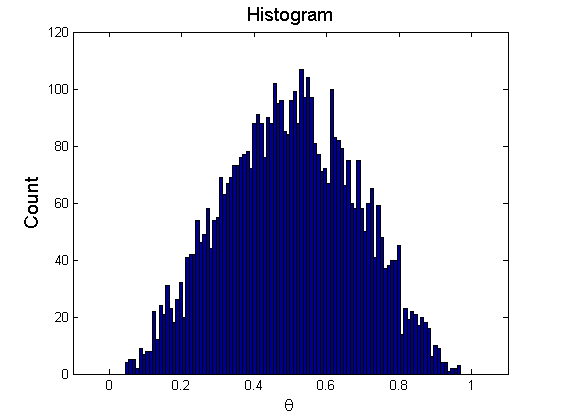
\includegraphics[scale=0.5]{GaussianHist.png}\\
\end{right}

\item\underline{Efficiency:}\\
In the case of Uniform density, we end up rejecting a lot of samples because they have equal probability of being drawn in the $[0,1]$ interval. Hence an efficient envelope density would be one that conforms to general shape of the target density. In this case, we do not end up rejecting a lot of samples drawn from $\mathcal{N}(0.5,0.04),$ because samples in $[0,1]$ have more or less similar probabilities of being drawn. Hence it is more efficient than Uniform.  
\end{enumerate}

\pagebreak
\noindent {\Large\underline{\textbf{Appendix:}}}\\
\lstinputlisting{C:/Users/ksp6/Documents/Classes/2013-Fall/STA601-BayesAndModStats/labs/lab4/sta601_ksp6_Lab4.m}

\end{document}